\documentclass[14pt]{extbook}
\usepackage{multicol, enumerate, enumitem, hyperref, color, soul, setspace, parskip, fancyhdr} %General Packages
\usepackage{amssymb, amsthm, amsmath, latexsym, units, mathtools} %Math Packages
\everymath{\displaystyle} %All math in Display Style
% Packages with additional options
\usepackage[headsep=0.5cm,headheight=12pt, left=1 in,right= 1 in,top= 1 in,bottom= 1 in]{geometry}
\usepackage[usenames,dvipsnames]{xcolor}
\usepackage{dashrule}  % Package to use the command below to create lines between items
\newcommand{\litem}[1]{\item#1\hspace*{-1cm}\rule{\textwidth}{0.4pt}}
\pagestyle{fancy}
\lhead{Makeup Progress Quiz 2}
\chead{}
\rhead{Version ALL}
\lfoot{2790-1423}
\cfoot{}
\rfoot{Summer C 2021}
\begin{document}

\begin{enumerate}
\litem{
Which of the following equations \textit{could} be of the graph presented below?
\begin{center}
    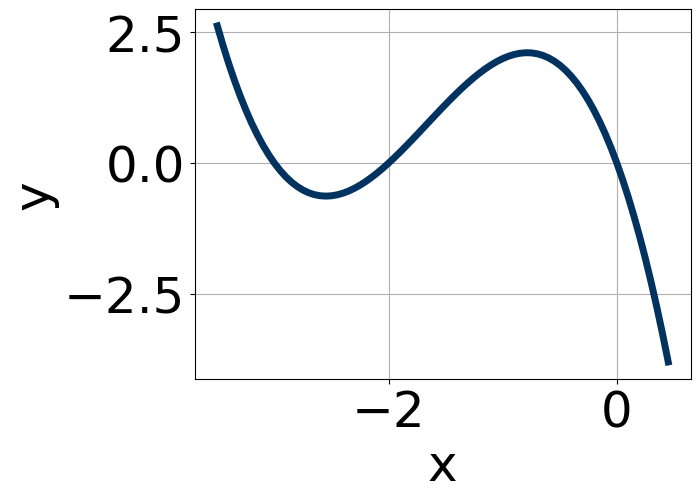
\includegraphics[width=0.5\textwidth]{../Figures/polyGraphToFunctionA.png}
\end{center}
\begin{enumerate}[label=\Alph*.]
\item \( -19x^{11} (x + 2)^{9} (x + 3)^{9} \)
\item \( 8x^{7} (x + 2)^{11} (x + 3)^{9} \)
\item \( -2x^{9} (x + 2)^{10} (x + 3)^{8} \)
\item \( -19x^{5} (x + 2)^{8} (x + 3)^{9} \)
\item \( 15x^{9} (x + 2)^{6} (x + 3)^{7} \)

\end{enumerate} }
\litem{
Construct the lowest-degree polynomial given the zeros below. Then, choose the intervals that contain the coefficients of the polynomial in the form $ax^3+bx^2+cx+d$.\[ \frac{-3}{2}, -7, \text{ and } \frac{7}{2} \]\begin{enumerate}[label=\Alph*.]
\item \( a \in [1, 7], b \in [20, 23], c \in [-77, -71], \text{ and } d \in [-149, -143] \)
\item \( a \in [1, 7], b \in [-20, -13], c \in [-77, -71], \text{ and } d \in [147, 150] \)
\item \( a \in [1, 7], b \in [6, 15], c \in [-120, -118], \text{ and } d \in [147, 150] \)
\item \( a \in [1, 7], b \in [20, 23], c \in [-77, -71], \text{ and } d \in [147, 150] \)
\item \( a \in [1, 7], b \in [-52, -47], c \in [158, 164], \text{ and } d \in [-149, -143] \)

\end{enumerate} }
\litem{
Describe the zero behavior of the zero $x = -7$ of the polynomial below.\[ f(x) = -2(x - 4)^{8}(x + 4)^{5}(x + 7)^{10}(x - 7)^{9} \]\begin{enumerate}[label=\Alph*.]
\begin{multicols}{2}\item 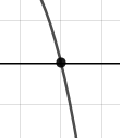
\includegraphics[width = 0.3\textwidth]{../Figures/polyZeroBehaviorCopyAA.png}\item 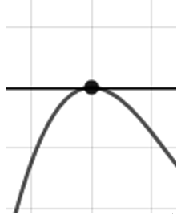
\includegraphics[width = 0.3\textwidth]{../Figures/polyZeroBehaviorCopyBA.png}\item 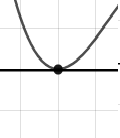
\includegraphics[width = 0.3\textwidth]{../Figures/polyZeroBehaviorCopyCA.png}\item 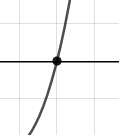
\includegraphics[width = 0.3\textwidth]{../Figures/polyZeroBehaviorCopyDA.png}\end{multicols}\item None of the above.
\end{enumerate} }
\litem{
Describe the end behavior of the polynomial below.\[ f(x) = 7(x - 7)^{2}(x + 7)^{3}(x - 8)^{5}(x + 8)^{5} \]\begin{enumerate}[label=\Alph*.]
\begin{multicols}{2}\item 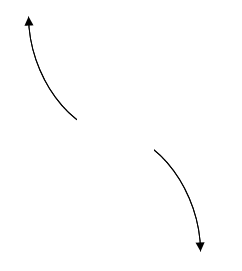
\includegraphics[width = 0.3\textwidth]{../Figures/polyEndBehaviorCopyAA.png}\item 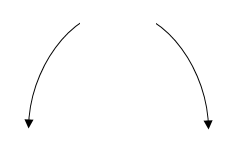
\includegraphics[width = 0.3\textwidth]{../Figures/polyEndBehaviorCopyBA.png}\item 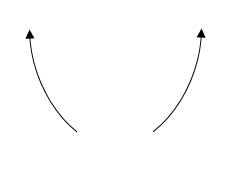
\includegraphics[width = 0.3\textwidth]{../Figures/polyEndBehaviorCopyCA.png}\item 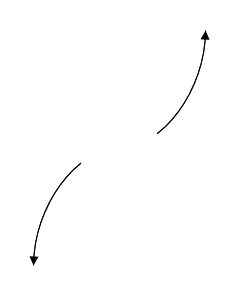
\includegraphics[width = 0.3\textwidth]{../Figures/polyEndBehaviorCopyDA.png}\end{multicols}\item None of the above.
\end{enumerate} }
\litem{
Describe the end behavior of the polynomial below.\[ f(x) = 2(x - 2)^{4}(x + 2)^{7}(x - 4)^{2}(x + 4)^{2} \]\begin{enumerate}[label=\Alph*.]
\begin{multicols}{2}\item 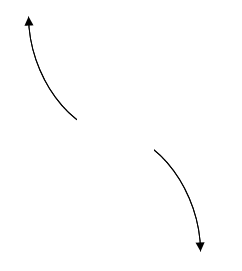
\includegraphics[width = 0.3\textwidth]{../Figures/polyEndBehaviorAA.png}\item 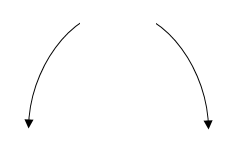
\includegraphics[width = 0.3\textwidth]{../Figures/polyEndBehaviorBA.png}\item 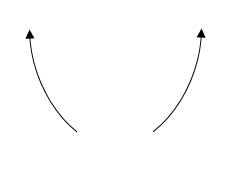
\includegraphics[width = 0.3\textwidth]{../Figures/polyEndBehaviorCA.png}\item 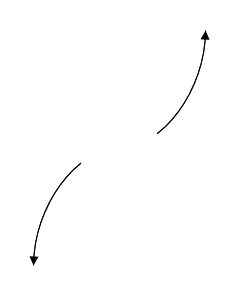
\includegraphics[width = 0.3\textwidth]{../Figures/polyEndBehaviorDA.png}\end{multicols}\item None of the above.
\end{enumerate} }
\litem{
Construct the lowest-degree polynomial given the zeros below. Then, choose the intervals that contain the coefficients of the polynomial in the form $x^3+bx^2+cx+d$.\[ -4 + 4 i \text{ and } 4 \]\begin{enumerate}[label=\Alph*.]
\item \( b \in [0.9, 3.2], c \in [-3, 3], \text{ and } d \in [-18, -14] \)
\item \( b \in [0.9, 3.2], c \in [-10, -7], \text{ and } d \in [13, 21] \)
\item \( b \in [-7.8, -3.9], c \in [-3, 3], \text{ and } d \in [121, 134] \)
\item \( b \in [3.1, 5.5], c \in [-3, 3], \text{ and } d \in [-130, -123] \)
\item \( \text{None of the above.} \)

\end{enumerate} }
\litem{
Construct the lowest-degree polynomial given the zeros below. Then, choose the intervals that contain the coefficients of the polynomial in the form $ax^3+bx^2+cx+d$.\[ -3, \frac{-5}{2}, \text{ and } \frac{-1}{5} \]\begin{enumerate}[label=\Alph*.]
\item \( a \in [10, 15], b \in [51, 61], c \in [80, 87], \text{ and } d \in [11, 19] \)
\item \( a \in [10, 15], b \in [-53, -46], c \in [53, 71], \text{ and } d \in [11, 19] \)
\item \( a \in [10, 15], b \in [-57, -54], c \in [80, 87], \text{ and } d \in [-17, -7] \)
\item \( a \in [10, 15], b \in [-3, 6], c \in [-81, -75], \text{ and } d \in [-17, -7] \)
\item \( a \in [10, 15], b \in [51, 61], c \in [80, 87], \text{ and } d \in [-17, -7] \)

\end{enumerate} }
\litem{
Which of the following equations \textit{could} be of the graph presented below?
\begin{center}
    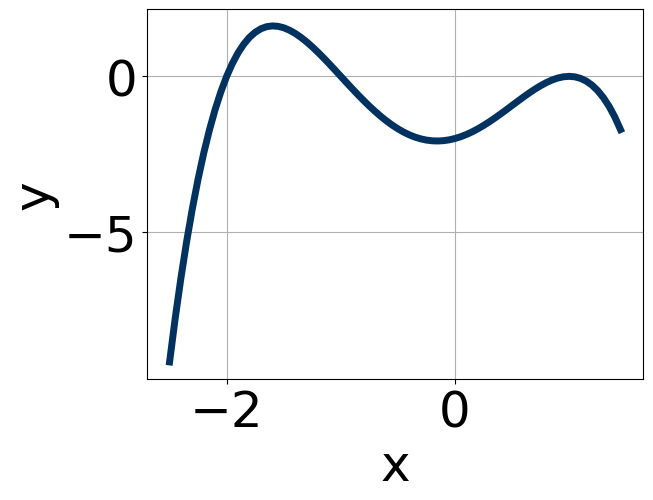
\includegraphics[width=0.5\textwidth]{../Figures/polyGraphToFunctionCopyA.png}
\end{center}
\begin{enumerate}[label=\Alph*.]
\item \( -15(x - 1)^{8} (x + 1)^{11} (x + 2)^{7} \)
\item \( -11(x - 1)^{8} (x + 1)^{6} (x + 2)^{9} \)
\item \( 16(x - 1)^{8} (x + 1)^{9} (x + 2)^{11} \)
\item \( -14(x - 1)^{7} (x + 1)^{8} (x + 2)^{9} \)
\item \( 11(x - 1)^{4} (x + 1)^{11} (x + 2)^{4} \)

\end{enumerate} }
\litem{
Construct the lowest-degree polynomial given the zeros below. Then, choose the intervals that contain the coefficients of the polynomial in the form $x^3+bx^2+cx+d$.\[ -3 - 4 i \text{ and } -2 \]\begin{enumerate}[label=\Alph*.]
\item \( b \in [-1, 5], c \in [1.8, 5.3], \text{ and } d \in [5.8, 6.4] \)
\item \( b \in [-1, 5], c \in [5.2, 8.8], \text{ and } d \in [7.7, 10.7] \)
\item \( b \in [4, 9], c \in [35.8, 38.9], \text{ and } d \in [46.8, 52.1] \)
\item \( b \in [-9, -3], c \in [35.8, 38.9], \text{ and } d \in [-50.4, -49] \)
\item \( \text{None of the above.} \)

\end{enumerate} }
\litem{
Describe the zero behavior of the zero $x = -8$ of the polynomial below.\[ f(x) = -2(x - 8)^{8}(x + 8)^{11}(x + 9)^{9}(x - 9)^{13} \]\begin{enumerate}[label=\Alph*.]
\begin{multicols}{2}\item 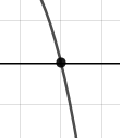
\includegraphics[width = 0.3\textwidth]{../Figures/polyZeroBehaviorAA.png}\item 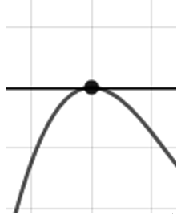
\includegraphics[width = 0.3\textwidth]{../Figures/polyZeroBehaviorBA.png}\item 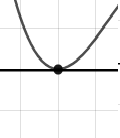
\includegraphics[width = 0.3\textwidth]{../Figures/polyZeroBehaviorCA.png}\item 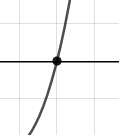
\includegraphics[width = 0.3\textwidth]{../Figures/polyZeroBehaviorDA.png}\end{multicols}\item None of the above.
\end{enumerate} }
\litem{
Which of the following equations \textit{could} be of the graph presented below?
\begin{center}
    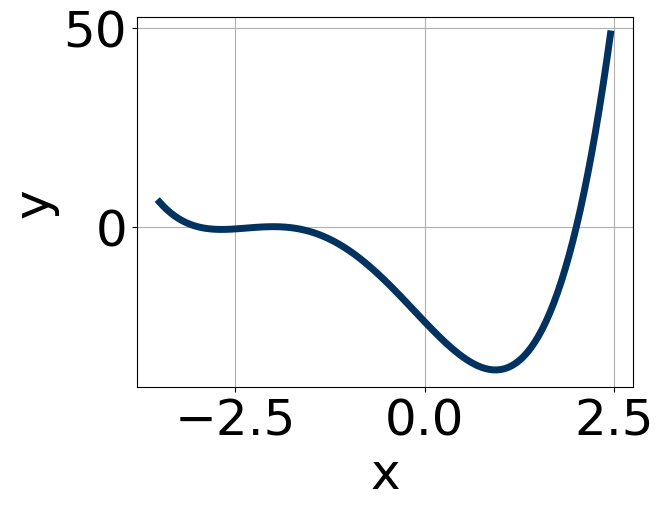
\includegraphics[width=0.5\textwidth]{../Figures/polyGraphToFunctionB.png}
\end{center}
\begin{enumerate}[label=\Alph*.]
\item \( 19(x + 2)^{7} (x - 2)^{4} (x + 3)^{9} \)
\item \( 20(x + 2)^{10} (x - 2)^{8} (x + 3)^{7} \)
\item \( 13(x + 2)^{4} (x - 2)^{11} (x + 3)^{11} \)
\item \( -18(x + 2)^{4} (x - 2)^{7} (x + 3)^{4} \)
\item \( -4(x + 2)^{10} (x - 2)^{11} (x + 3)^{5} \)

\end{enumerate} }
\litem{
Construct the lowest-degree polynomial given the zeros below. Then, choose the intervals that contain the coefficients of the polynomial in the form $ax^3+bx^2+cx+d$.\[ \frac{1}{4}, \frac{7}{5}, \text{ and } 2 \]\begin{enumerate}[label=\Alph*.]
\item \( a \in [17, 26], b \in [68, 75], c \in [69, 74], \text{ and } d \in [10, 16] \)
\item \( a \in [17, 26], b \in [-7, -6], c \in [-59, -56], \text{ and } d \in [-18, -13] \)
\item \( a \in [17, 26], b \in [-73, -66], c \in [69, 74], \text{ and } d \in [-18, -13] \)
\item \( a \in [17, 26], b \in [-73, -66], c \in [69, 74], \text{ and } d \in [10, 16] \)
\item \( a \in [17, 26], b \in [-66, -58], c \in [34, 45], \text{ and } d \in [10, 16] \)

\end{enumerate} }
\litem{
Describe the zero behavior of the zero $x = 2$ of the polynomial below.\[ f(x) = -9(x - 7)^{7}(x + 7)^{4}(x - 2)^{12}(x + 2)^{9} \]\begin{enumerate}[label=\Alph*.]
\begin{multicols}{2}\item 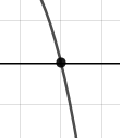
\includegraphics[width = 0.3\textwidth]{../Figures/polyZeroBehaviorCopyAB.png}\item 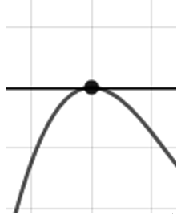
\includegraphics[width = 0.3\textwidth]{../Figures/polyZeroBehaviorCopyBB.png}\item 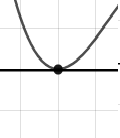
\includegraphics[width = 0.3\textwidth]{../Figures/polyZeroBehaviorCopyCB.png}\item 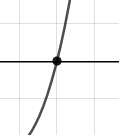
\includegraphics[width = 0.3\textwidth]{../Figures/polyZeroBehaviorCopyDB.png}\end{multicols}\item None of the above.
\end{enumerate} }
\litem{
Describe the end behavior of the polynomial below.\[ f(x) = 8(x - 9)^{2}(x + 9)^{5}(x - 7)^{4}(x + 7)^{6} \]\begin{enumerate}[label=\Alph*.]
\begin{multicols}{2}\item 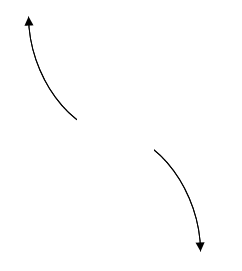
\includegraphics[width = 0.3\textwidth]{../Figures/polyEndBehaviorCopyAB.png}\item 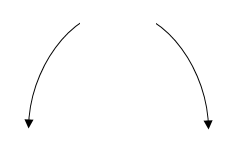
\includegraphics[width = 0.3\textwidth]{../Figures/polyEndBehaviorCopyBB.png}\item 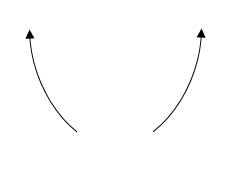
\includegraphics[width = 0.3\textwidth]{../Figures/polyEndBehaviorCopyCB.png}\item 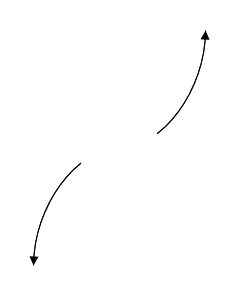
\includegraphics[width = 0.3\textwidth]{../Figures/polyEndBehaviorCopyDB.png}\end{multicols}\item None of the above.
\end{enumerate} }
\litem{
Describe the end behavior of the polynomial below.\[ f(x) = 9(x + 5)^{3}(x - 5)^{6}(x - 3)^{5}(x + 3)^{7} \]\begin{enumerate}[label=\Alph*.]
\begin{multicols}{2}\item 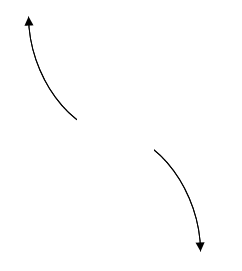
\includegraphics[width = 0.3\textwidth]{../Figures/polyEndBehaviorAB.png}\item 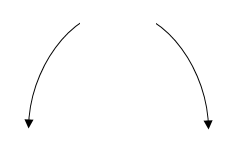
\includegraphics[width = 0.3\textwidth]{../Figures/polyEndBehaviorBB.png}\item 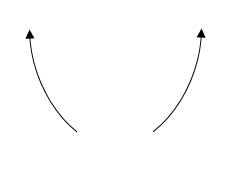
\includegraphics[width = 0.3\textwidth]{../Figures/polyEndBehaviorCB.png}\item 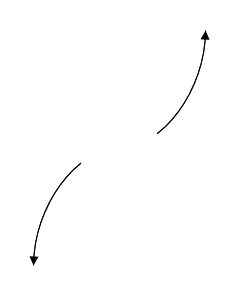
\includegraphics[width = 0.3\textwidth]{../Figures/polyEndBehaviorDB.png}\end{multicols}\item None of the above.
\end{enumerate} }
\litem{
Construct the lowest-degree polynomial given the zeros below. Then, choose the intervals that contain the coefficients of the polynomial in the form $x^3+bx^2+cx+d$.\[ -2 + 5 i \text{ and } 3 \]\begin{enumerate}[label=\Alph*.]
\item \( b \in [-0.1, 2.4], c \in [15, 24], \text{ and } d \in [-94, -80] \)
\item \( b \in [-2.5, -0.9], c \in [15, 24], \text{ and } d \in [75, 89] \)
\item \( b \in [-0.1, 2.4], c \in [-8, -3], \text{ and } d \in [10, 24] \)
\item \( b \in [-0.1, 2.4], c \in [-2, 5], \text{ and } d \in [-10, -2] \)
\item \( \text{None of the above.} \)

\end{enumerate} }
\litem{
Construct the lowest-degree polynomial given the zeros below. Then, choose the intervals that contain the coefficients of the polynomial in the form $ax^3+bx^2+cx+d$.\[ \frac{-3}{2}, \frac{-7}{3}, \text{ and } -4 \]\begin{enumerate}[label=\Alph*.]
\item \( a \in [1, 13], b \in [42, 51], c \in [111, 117], \text{ and } d \in [-87, -83] \)
\item \( a \in [1, 13], b \in [-4, 2], c \in [-76, -68], \text{ and } d \in [84, 88] \)
\item \( a \in [1, 13], b \in [-50, -41], c \in [111, 117], \text{ and } d \in [-87, -83] \)
\item \( a \in [1, 13], b \in [42, 51], c \in [111, 117], \text{ and } d \in [84, 88] \)
\item \( a \in [1, 13], b \in [28, 30], c \in [-3, 5], \text{ and } d \in [-87, -83] \)

\end{enumerate} }
\litem{
Which of the following equations \textit{could} be of the graph presented below?
\begin{center}
    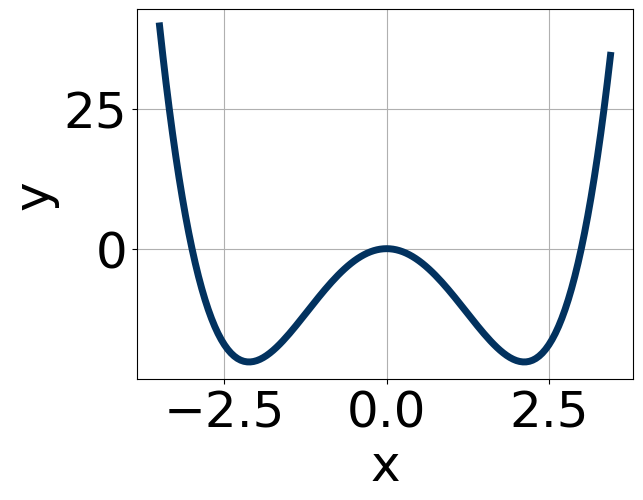
\includegraphics[width=0.5\textwidth]{../Figures/polyGraphToFunctionCopyB.png}
\end{center}
\begin{enumerate}[label=\Alph*.]
\item \( 18x^{8} (x + 3)^{9} (x - 3)^{7} \)
\item \( -19x^{4} (x + 3)^{5} (x - 3)^{4} \)
\item \( 19x^{4} (x + 3)^{8} (x - 3)^{11} \)
\item \( 8x^{5} (x + 3)^{8} (x - 3)^{7} \)
\item \( -3x^{4} (x + 3)^{11} (x - 3)^{7} \)

\end{enumerate} }
\litem{
Construct the lowest-degree polynomial given the zeros below. Then, choose the intervals that contain the coefficients of the polynomial in the form $x^3+bx^2+cx+d$.\[ 5 + 2 i \text{ and } 4 \]\begin{enumerate}[label=\Alph*.]
\item \( b \in [-6, 2], c \in [-9.4, -7.5], \text{ and } d \in [18, 22] \)
\item \( b \in [-21, -8], c \in [67.5, 70.9], \text{ and } d \in [-126, -113] \)
\item \( b \in [-6, 2], c \in [-8, -3.8], \text{ and } d \in [5, 12] \)
\item \( b \in [12, 21], c \in [67.5, 70.9], \text{ and } d \in [115, 119] \)
\item \( \text{None of the above.} \)

\end{enumerate} }
\litem{
Describe the zero behavior of the zero $x = 2$ of the polynomial below.\[ f(x) = 8(x + 2)^{2}(x - 2)^{7}(x - 4)^{9}(x + 4)^{11} \]\begin{enumerate}[label=\Alph*.]
\begin{multicols}{2}\item 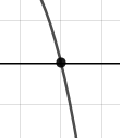
\includegraphics[width = 0.3\textwidth]{../Figures/polyZeroBehaviorAB.png}\item 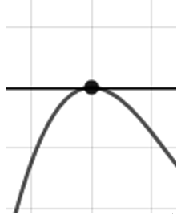
\includegraphics[width = 0.3\textwidth]{../Figures/polyZeroBehaviorBB.png}\item 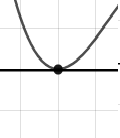
\includegraphics[width = 0.3\textwidth]{../Figures/polyZeroBehaviorCB.png}\item 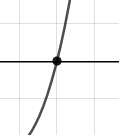
\includegraphics[width = 0.3\textwidth]{../Figures/polyZeroBehaviorDB.png}\end{multicols}\item None of the above.
\end{enumerate} }
\litem{
Which of the following equations \textit{could} be of the graph presented below?
\begin{center}
    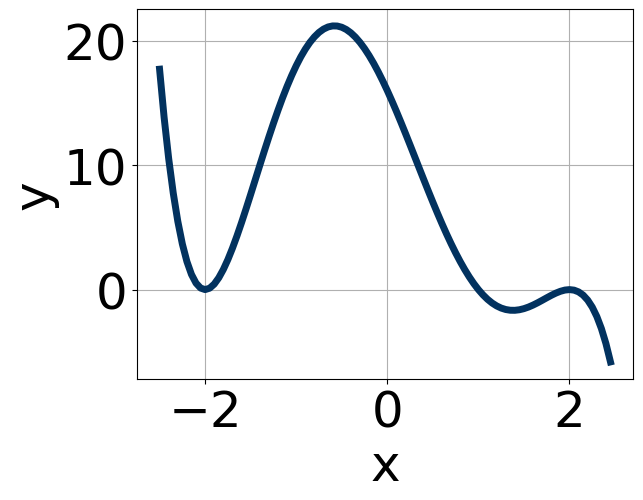
\includegraphics[width=0.5\textwidth]{../Figures/polyGraphToFunctionC.png}
\end{center}
\begin{enumerate}[label=\Alph*.]
\item \( -13(x - 2)^{10} (x + 2)^{5} (x - 1)^{10} \)
\item \( -14(x - 2)^{10} (x + 2)^{9} (x - 1)^{11} \)
\item \( 18(x - 2)^{10} (x + 2)^{4} (x - 1)^{10} \)
\item \( -6(x - 2)^{10} (x + 2)^{4} (x - 1)^{7} \)
\item \( 16(x - 2)^{8} (x + 2)^{8} (x - 1)^{5} \)

\end{enumerate} }
\litem{
Construct the lowest-degree polynomial given the zeros below. Then, choose the intervals that contain the coefficients of the polynomial in the form $ax^3+bx^2+cx+d$.\[ \frac{-3}{5}, \frac{7}{4}, \text{ and } \frac{1}{3} \]\begin{enumerate}[label=\Alph*.]
\item \( a \in [53, 63], b \in [-91, -78], c \in [-46, -37], \text{ and } d \in [-21, -18] \)
\item \( a \in [53, 63], b \in [-91, -78], c \in [-46, -37], \text{ and } d \in [20, 23] \)
\item \( a \in [53, 63], b \in [83, 95], c \in [-46, -37], \text{ and } d \in [-21, -18] \)
\item \( a \in [53, 63], b \in [49, 51], c \in [-88, -79], \text{ and } d \in [20, 23] \)
\item \( a \in [53, 63], b \in [-165, -159], c \in [107, 112], \text{ and } d \in [-21, -18] \)

\end{enumerate} }
\litem{
Describe the zero behavior of the zero $x = 8$ of the polynomial below.\[ f(x) = 3(x + 8)^{8}(x - 8)^{11}(x - 7)^{9}(x + 7)^{13} \]\begin{enumerate}[label=\Alph*.]
\begin{multicols}{2}\item 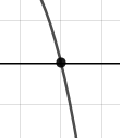
\includegraphics[width = 0.3\textwidth]{../Figures/polyZeroBehaviorCopyAC.png}\item 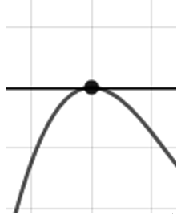
\includegraphics[width = 0.3\textwidth]{../Figures/polyZeroBehaviorCopyBC.png}\item 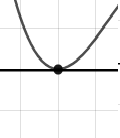
\includegraphics[width = 0.3\textwidth]{../Figures/polyZeroBehaviorCopyCC.png}\item 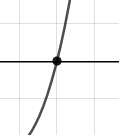
\includegraphics[width = 0.3\textwidth]{../Figures/polyZeroBehaviorCopyDC.png}\end{multicols}\item None of the above.
\end{enumerate} }
\litem{
Describe the end behavior of the polynomial below.\[ f(x) = -4(x + 6)^{4}(x - 6)^{5}(x + 2)^{5}(x - 2)^{5} \]\begin{enumerate}[label=\Alph*.]
\begin{multicols}{2}\item 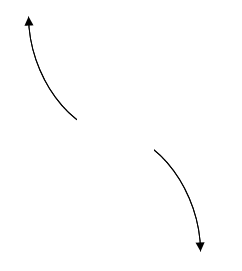
\includegraphics[width = 0.3\textwidth]{../Figures/polyEndBehaviorCopyAC.png}\item 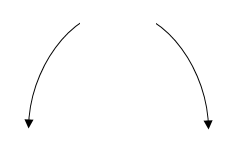
\includegraphics[width = 0.3\textwidth]{../Figures/polyEndBehaviorCopyBC.png}\item 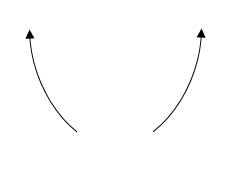
\includegraphics[width = 0.3\textwidth]{../Figures/polyEndBehaviorCopyCC.png}\item 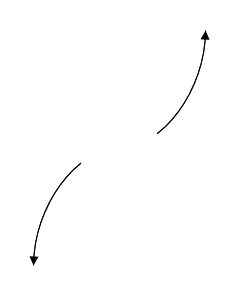
\includegraphics[width = 0.3\textwidth]{../Figures/polyEndBehaviorCopyDC.png}\end{multicols}\item None of the above.
\end{enumerate} }
\litem{
Describe the end behavior of the polynomial below.\[ f(x) = 4(x + 2)^{5}(x - 2)^{8}(x + 9)^{3}(x - 9)^{3} \]\begin{enumerate}[label=\Alph*.]
\begin{multicols}{2}\item 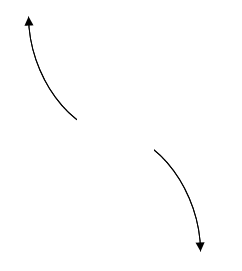
\includegraphics[width = 0.3\textwidth]{../Figures/polyEndBehaviorAC.png}\item 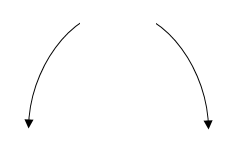
\includegraphics[width = 0.3\textwidth]{../Figures/polyEndBehaviorBC.png}\item 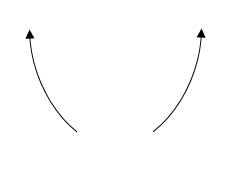
\includegraphics[width = 0.3\textwidth]{../Figures/polyEndBehaviorCC.png}\item 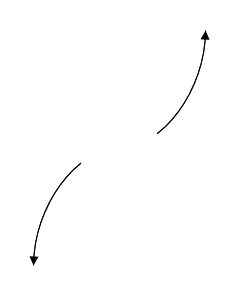
\includegraphics[width = 0.3\textwidth]{../Figures/polyEndBehaviorDC.png}\end{multicols}\item None of the above.
\end{enumerate} }
\litem{
Construct the lowest-degree polynomial given the zeros below. Then, choose the intervals that contain the coefficients of the polynomial in the form $x^3+bx^2+cx+d$.\[ -5 + 5 i \text{ and } -1 \]\begin{enumerate}[label=\Alph*.]
\item \( b \in [-16, -10], c \in [59, 67], \text{ and } d \in [-58, -48] \)
\item \( b \in [4, 19], c \in [59, 67], \text{ and } d \in [46, 58] \)
\item \( b \in [-8, 6], c \in [-1, 13], \text{ and } d \in [3, 6] \)
\item \( b \in [-8, 6], c \in [-6, 3], \text{ and } d \in [-7, 3] \)
\item \( \text{None of the above.} \)

\end{enumerate} }
\litem{
Construct the lowest-degree polynomial given the zeros below. Then, choose the intervals that contain the coefficients of the polynomial in the form $ax^3+bx^2+cx+d$.\[ \frac{-2}{5}, \frac{-3}{2}, \text{ and } \frac{1}{5} \]\begin{enumerate}[label=\Alph*.]
\item \( a \in [48, 62], b \in [44, 50], c \in [-44, -38], \text{ and } d \in [1, 10] \)
\item \( a \in [48, 62], b \in [-106, -98], c \in [42, 50], \text{ and } d \in [-8, 2] \)
\item \( a \in [48, 62], b \in [79, 88], c \in [7, 18], \text{ and } d \in [-8, 2] \)
\item \( a \in [48, 62], b \in [79, 88], c \in [7, 18], \text{ and } d \in [1, 10] \)
\item \( a \in [48, 62], b \in [-85, -84], c \in [7, 18], \text{ and } d \in [1, 10] \)

\end{enumerate} }
\litem{
Which of the following equations \textit{could} be of the graph presented below?
\begin{center}
    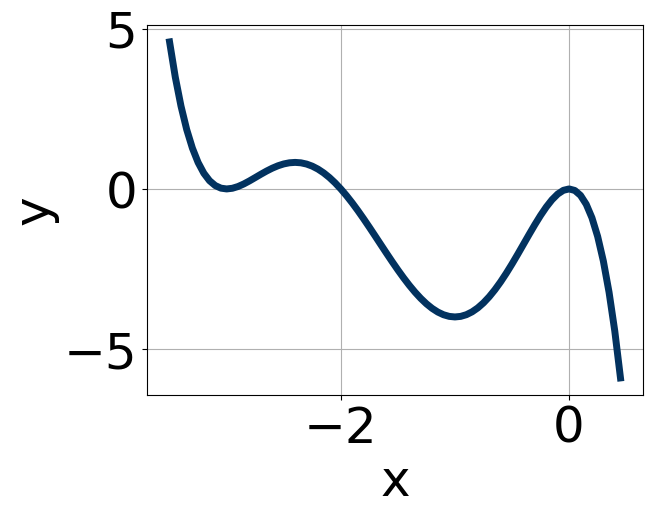
\includegraphics[width=0.5\textwidth]{../Figures/polyGraphToFunctionCopyC.png}
\end{center}
\begin{enumerate}[label=\Alph*.]
\item \( 14x^{10} (x + 3)^{10} (x + 2)^{5} \)
\item \( 18x^{10} (x + 3)^{4} (x + 2)^{4} \)
\item \( -11x^{9} (x + 3)^{6} (x + 2)^{5} \)
\item \( -13x^{8} (x + 3)^{10} (x + 2)^{5} \)
\item \( -8x^{11} (x + 3)^{10} (x + 2)^{10} \)

\end{enumerate} }
\litem{
Construct the lowest-degree polynomial given the zeros below. Then, choose the intervals that contain the coefficients of the polynomial in the form $x^3+bx^2+cx+d$.\[ 4 - 3 i \text{ and } 3 \]\begin{enumerate}[label=\Alph*.]
\item \( b \in [9, 12], c \in [40, 52], \text{ and } d \in [74, 86] \)
\item \( b \in [-14, -5], c \in [40, 52], \text{ and } d \in [-77, -72] \)
\item \( b \in [0, 3], c \in [0, 5], \text{ and } d \in [-9, -8] \)
\item \( b \in [0, 3], c \in [-10, -6], \text{ and } d \in [7, 16] \)
\item \( \text{None of the above.} \)

\end{enumerate} }
\litem{
Describe the zero behavior of the zero $x = 3$ of the polynomial below.\[ f(x) = 3(x - 3)^{5}(x + 3)^{10}(x + 8)^{5}(x - 8)^{6} \]\begin{enumerate}[label=\Alph*.]
\begin{multicols}{2}\item \includegraphics[width = 0.3\textwidth]{../Figures/polyZeroBehaviorAC.png}\item \includegraphics[width = 0.3\textwidth]{../Figures/polyZeroBehaviorBC.png}\item \includegraphics[width = 0.3\textwidth]{../Figures/polyZeroBehaviorCC.png}\item \includegraphics[width = 0.3\textwidth]{../Figures/polyZeroBehaviorDC.png}\end{multicols}\item None of the above.
\end{enumerate} }
\end{enumerate}

\end{document}